\documentclass[english]{article}
\usepackage[T1]{fontenc}
\usepackage[latin9]{inputenc}
\usepackage{graphicx}
\usepackage{listings}
\usepackage{geometry}
\geometry{verbose,tmargin=1.47cm,bmargin=1.47cm,lmargin=1.47cm,rmargin=1.47cm}

\makeatletter
\pagestyle{empty}
\usepackage{tikz}
\usetikzlibrary{arrows,shadows} % for pgf-umlsd
\usepackage[underline=true,rounded corners=false]{pgf-umlsd}

\makeatother

\usepackage{babel}
\begin{document}

\title{BSOS}


\author{Alexander Gould, William Woodruff, Pawe\l{} Czarnecki, Reyna Shaskan}


\date{Post-AP Robotics Final Project}
\maketitle
\begin{abstract}
For our final project, we decided to play around with low level programming
and system design, so we decided to make our own operating system
for the Cortex! It's inspired by {*}NIX systems, and runs on x86 processors
(like the ones on our computers) and ARM processors (like the ones
in the Cortex). It has support for traditional keyboard input and
screen output and is also able to interface with the motors and sensors
on the VeX system. It bosts far less bloat and faster response time
than the pre-loaded OS on the Cortex. It's called BSOS because the
letters sound nice and stand for Bronx Science and not for any other reason whatsoever.
\end{abstract}

\part{Operating System Basics-Reyna}
\paragraph{Theory}
An Operating System has several different components. All software has to go through the OS in order for the user to be able to utilize any of the hardware. The kernel offers a basic level of control over doing this. The kernel manages memory access for programs in the RAM, determines which programs connect with which hardware, handles the CPU's operating states, organizes data in the long run, and orders processes in multi-tasking systems. Essentially, the kernel assigns memory space.

\paragraph{Interrupts}
Interrupts are also very important. Interrupts create an efficient way for the OS to interact with its environment. Older systems used to monitor different sources of input for events. Interrupts help automatically save local register contexts and run particular code in response to particular events. Interrupts cause the current program to pause for a moment, save it, and then run code associated with that interrupt. In other words, an interrupt interrupts the program-hence the name. Interupts are handles by the kernel.

\paragraph{Types}
Three different types of interrupts are hardware interrupts, software interrupts, and traps. Hardware interrupts may come from a key on a keyboard being hit or the click of a mouse. Software interrupts are generated by programs. Traps come from the CPU itself due to errors or conditions which require the OS for assistance.

\paragraph{Boot}
When a computer initially turns on, it runs in supervisor mode. The first programs to run have unlimited access to hardware. When the OS allows another program to take control, the computer transitions into protected mode, where programs' access to the CPU's set of instructions is limited. To leave protected mode, an interrupt has to be triggered so that way the kernel will be able to take charge once again.

\paragraph{Summary}
An OS manages the interactions between hardware and software on the computer. The most common Operating Systems are Microsoft Windows, Mac OS X, and Linux.

\part{Booting Up-William}
BSOS, as a portable and abstracted system, must be capable of bootstrapping on a variety of diverse and divergent architectures. Although hundreds exist, ranging from giants like x86, POWER, and ARM to lesser known embedded architectures like AVR and MIPS, the vast majority of fall into one of two families: CISC and RISC.

CISC, or Complex Instruction Set Computing, began as a side effect of early computer development. As the (comparatively primitive) computers and calculators of the 1950s and 1960s became increasingly complex and multifunctional, they required new paradigms and methods of automation. Because languages like FORTRAN and ALGOL required a certain amount of boilerplate in order to operate, early system architects build complex control structures into the instruction sets of their machines, bridging the semantic gap between microcode-assembly and full-features programming languages.

\paragraph{x86}
On x86 machines, specifically i386 and later, BSOS begins in 16-bit real mode. The strapping sector, which is 512 bytes long, then loads a general descriptor table, or GDT, into memory. That descriptor table is then used to switch the CPU into 32-bit protected mode, whereupon the kernel is loaded.
\begin{figure}[h!]
\centerline{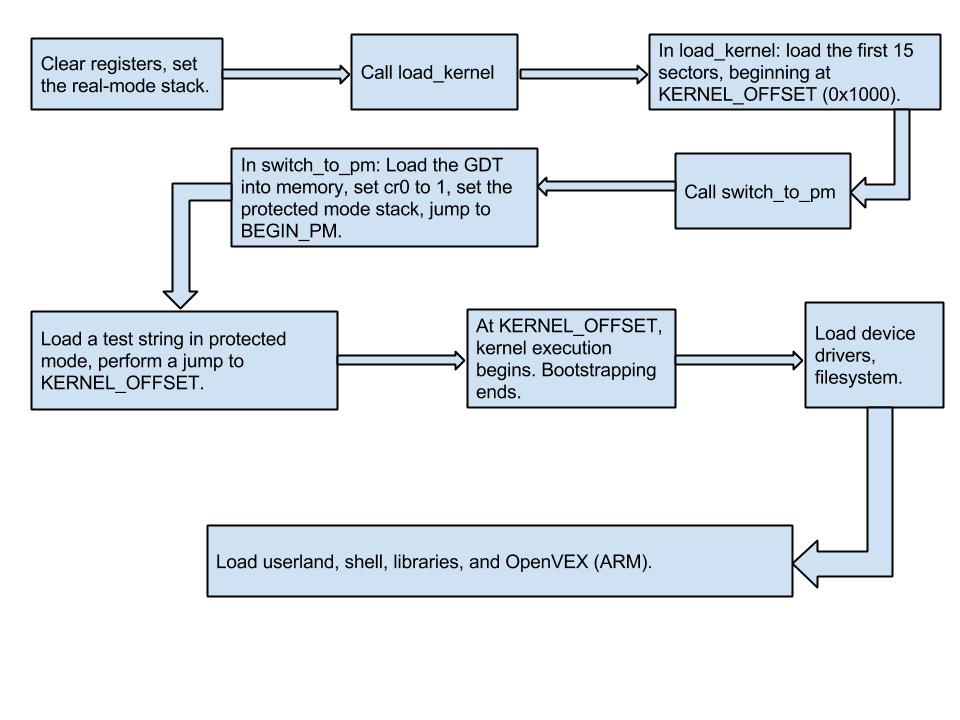
\includegraphics[scale=0.4]{imgs/boot_x86.png}}
\caption{Figure 1: Bootstrapping on i386.}
\end{figure}

\paragraph{ARM}
On ARM-based machines, specifically those with Cortex-M3 processors, the bootstrapping process is remarkably similar. Despite the RISC (Reduced Instruction Set Computing) nature of the ARM architecture


\part{Memory Management- Pawe\l{}}

\paragraph{Introduction}
In all modern computer systems arrises the necessesity to manage resources, in particular memory. Because a typical general purpose computer
may have many different programs running simulatneously it is crucial to have a subsystem that assigns memory regions to applications and keeps
track of those regions. In the case of modern operating systems the implementation of such a system may be done so based on different principles.
In a very simple Operating System which is responsible for managing resources for a small pool of applications the choice of paradigm does not have a large impact on system stability or performance.
With simpliciy taken into account, the BSOS memory management system assigns variable sized blocks of memory to applications and keeps track of their status.


\part{Interfacing With Hardware-Alex}
There are 2 main components to input and output for this operating system, keyboard and screen, and motors and sensors.
\paragraph{Keyboard and Screen}
Information is se4nt from the keyboard to the processor via a standard protocol. Inside any commercial keyboard is a tiny computer chip
called a {\it microcontroller}. When a key is pressed down, the microcontroller receives the signal and starts a short countdown timer. If your finger is still pressing down on the key after more than a millisecond, the microcontroller looks up a numerical value for the key
and saves it in its small memory bank.
\break
\\The data is then sent to the computer along a cable, usually USB. At any given moment, power
is passing through this cable to supply power to the keyboard, as well as to synchronize the keyboards internal timer. When the
computer receives this data is sent to a program known as the {\it driver} for processing. The driver interprets this information
and sends it to the input stream of whatever program is currently running in the form of bytes, hexadecimal numbers representing
letters, symbols and punctuation marks. The program then processes the information in a way that makes sense, be that displaying
the symbol on a screen, saving it locally in a document, or interpretng it as a {\it control code}.
\break
\\A good example of this is the \texttt{CTRL+S} command. When you hold down the \texttt{CTRL} key, information is sent to the keyboard's onboard processor that that key is being held down. When you then press the \texttt{S} key, the numerical value for that key is sent for processing. The processor sees the code for the \texttt{S} key, but since the \texttt{CTRL} key is also held down, it changes the value sent to the computer to a control code. On your computer, the driver is monitoring continual packets of information sent in to the computer. Since the keyboard sends hundreds of these per second, most are empty. When one arrives with the control code you sent, the driver tells your operating system to process it. Your OS then tells your word processor. (Say it's your active window) When your word processor recieves this information, (Some OS'es will relay the control code directly, others will interpret it and send their own message) it then takes appropriate action and saves your document.
\break
\\The process works in reverse for display drivers. Since our OS uses a standard Video Graphics Array (VGA), I'll use that as an example.VGA monitors don't operate digitally like computers do, instead requiring a constant stream of electrons {\it analogous} to the image displayed, much like older TV's and radios. This poses a problem in that when programs send display data to your OS, your OS stores its images to output as digital files, long lists of discrete numbers. These two kinds of representing data don't play nice with each other, and it's the job of another driver to convert the signal.This driver takes the image, and splits it into red, green and blue elements, and stores it in its {\it video memory}. Think of the video memory as a canvas, a place where the driver draws what you see. After splitting the image into the three colors and drawing out each pixel as a combination of the three, the driver then sends the image as a set of analog signals, the same kind that travel to your cable box. For as long as the image in video memory remains unchanged, it keeps getting sent, and any changes to video memory are sent immediatley. Sending these signals continuously means that the image always stays on your monitor.
\break
\\Say we want to display a picture in the center of the screen. The program we use to do that, say ImageViewer or something, will take the picture data and send it to the OS in the form of digital values. How exactly depends on the image format and program you're using, but by the time the image gets to the OS, it's represented as a string of pixels. These pixels are then sent to the VGA driver, which breaks them down into red, green and blue values. Once that's done, it sends this information out through its pins in the form of analog signals, one color per pin, with extra pins used for time synchronization and error checking. These signals are directed via your monitor's onboard processor to their appropriate pixels, which light up in the colors you want. From a distance of a few inches, these colors blend to form your picture.
\paragraph{Sensors and Motors}
Information was originally sent from central control units to motors using a mechanism known as a {\it rheostat}. Basically, a rheostat was a long coil of wire. In order to get a motor to run at different speeds, current would be added at different points along the wire, and the amount of curent that wasn't dissipated by the wire drove the motor. While it was perfectly adequate in large machines, this approach doesn't work in robotics. While it's easy to set up, it takes up way too much space and dissipates way too much heat. 
\break
\\To solve this problem, modern servos use a system known as {\it Pulse Width Management} to regulate power sent to motors and sensors. The actual mechanics are somewhat complicated, but the principle itself is quite simple. Alternating current, as we know, can oscillate in many different patterns, triangle, square, sawtooth, what have you, but the most common form of oscillation is the simple quare wave, easy to convert to binary and simple to generate. What PWM does is power the motor with a quickly oscillating square wave AC current. In order to change the power supplied to the motor, the microcontroller varies the width of the pulses. In order to make the motor run faster, we make the "ON",or positive, portions of the wave longer, and the "OFF", or negative, portions shorter, raising the average value of the wave,which the motor interprets as more or less power. The opposite is true. By widening the "OFF" sections, we can slow the motor down. PWM also works for sensors. By sending back pulses of different widths, sensors can send us data about brightness, color or quantity. (Say, for a motor encoder.)
\break
\\Once all the drivers are in place and running, it's a simple matter to call their functionality from within the OS kernel, making the data sent and recieved readily usable by all programs on the device. (See Parts 1 and 3)

\end{document}
